\RequirePackage[l2tabu, orthodox]{nag}
\documentclass[11pt,a4paper,oneside,french]{report}
\pagestyle{plain}

\usepackage{standalone}
\usepackage{fixltx2e}
\usepackage{mathtools}
\usepackage{babel}
\usepackage{csquotes}
\usepackage{xspace}
%\usepackage{geometry}
%\usepackage[backend=biber, doi=false, url=false]{biblatex}
\usepackage{graphicx}
\usepackage{float}
\usepackage{subcaption}
\usepackage[justification=centering]{caption}
\usepackage[modulo]{lineno}			% N° de ligne dans \begin{linenumbers}
\usepackage{lipsum}					% Lorem ipsum dans \lipsum
\usepackage[autolanguage]{numprint} 	%Utilisation : \nombre{199999.999 e-17}
\usepackage[perpage]{footmisc}
\usepackage[all]{nowidow}
\usepackage{newclude}
\usepackage{booktabs}
\usepackage{tabu}
\usepackage{multicol}					%\begin{multicols}{<nbColonnes>}[<Texte avt colonne>]{<txt> \columnbreak <txt>}


\usepackage{fontspec}
\setmainfont[SmallCapsFont={Latin Modern Roman Caps},Ligatures=TeX]{Latin Modern Roman}
%\setmainfont[Ligatures=TeX]{Fira Sans}

\usepackage[hidelinks]{hyperref} 		%\href{<url>}{<text to display>}
\usepackage{microtype}


%\addbibresource{base.bib}
\title{\textsc{Titre}}
\author{Auteur}
\date{2000}


\begin{document}
	\begin{titlepage}
		\centering
		\vspace*{\baselineskip}
		\rule{\textwidth}{1.6pt}\vspace*{-\baselineskip}\vspace*{2pt}
		\rule{\textwidth}{0.4pt}\\[\baselineskip]
		{\LARGE\scshape La Communication Vibratoire}\\[0.2\baselineskip]
		\rule{\textwidth}{0.4pt}\vspace*{-\baselineskip}\vspace{3.2pt}
		\rule{\textwidth}{1.6pt}\\[\baselineskip]
		\scshape
		Que permettent les nouvelles connaissances en matière de communication animale ?\\
		\vspace*{2\baselineskip}
		Rédigé par \\[\baselineskip]
		{\Large Syrine BEL HAJ YAHIA \\ Valentin OGIER \\ Adam ROUGAGNOU\par}
		{\itshape Lycée Delacroix\par}
		\vfill
		{\scshape 2015} \\
		{\large}\par
	\end{titlepage}
	
	\thispagestyle{empty}
	\addtocounter{page}{-1}%
	\mbox{}
	
	\tableofcontents
	
	\setlength{\parskip}{2pt}%
	
	\section*{Introduction}
\addcontentsline{toc}{section}{\protect\numberline{}Introduction}%
Pour nous, humains, la communication repose principalement sur la
parole, sur l'utilisation d'une langue complexe, variée et en constante
évolution. C'est pourquoi il serait tentant de penser que notre mode de
communication est le plus développé du monde animal. Pourtant, en
s'intéressant aux modes de communication utilisés par les animaux, on

Il est logique de s'inspirer du comportement et des techniques des
animaux en matière de communication, étant donné que les espèces les
plus aptes à communiquer ont survécu, et leur technique de communication
est donc optimisé.

cf \url{http://s-f-walker.org.uk/pubsebooks/pdfs/animal-communication98.pdf}


	
	\chapter{La communication chimique}
\section{Les phéromones}
\subsection{Les Substances sémiochimiques}

Les substances sémiochimiques sont des molécules organiques synthétisées
par un organisme vivant et qui interviennent comme moyen de
communication que ce soit de manière intraspécifique ou de manière
interspécifique. Ces substances sémiochimiques modifie le comportement
ou la physiologie du récepteur.

TODO Image Les actions interspécifiques, ont lieu grâce aux substances
allélochimiques, ce sont des actions concernant les relations entre
différentes espèces alors que les actions intraspécifiques, ayant lieu
grâce aux phéromones sont relatif aux rapports qui se produisent au sein
d'une même espèce. C'est pour cette raison, que nous allons nous
intéresser aux phéromones pour étudier la communication chimique qui a
lieu au sein d'une même espèce, les fourmis.

\subsubsection{Définition de phéromone}

La notion de phéromone a été introduite par Karlson et Lüsher en 1959,
ils en ont donné la définition suivante : « Une phéromone est une
substance (ou un mélange de substances) qui, après avoir été sécrétée à
l'extérieur par un individu (émetteur), est perçue par un individu de la
même espèce (récepteur) chez lequel elle provoque une réaction
comportementale spécifique, voire une modification physiologique. »Le
mot phéromone vient du grec pherein « transporter » et hormân «exciter
». Les phéromones sont produites par des glandes spécifiques et sont
secrétées à l'extérieur d'un organisme. Comme les enzymes, elles
agissent dans des quantités minimes. Nous allons étudier un peu plus
tard ces glandes spécifiques dans la partie émission.

Généralement ; on ne parle pas d'une seule phéromone mais plutôt d'un
bouquet phéromonale. En effet ; les phéromones ne sont pas des corps
purs mais des mélanges de différentes substances chimiques. Le message
transmis est spécifique aux autres fourmis, ainsi sa composition de
point de vue qualitatif mais aussi quantitatif prend tout son sens.

\subsubsection{Les différents types de phéromones :}

Le célèbre scientifique Wilson, en 1962, distingue les phéromones de
déclanchement aux phéromones modificatrices selon leurs modes d'action.
Selon lui : - « Les phéromones de déclanchement produisent un changement
d'état immédiat et réversible dans le comportement du récepteur ». Il y
classe les phéromones sexuelles (attractives ou aphrodisiaques), les
phéromones d'alarme, les phéromones de piste, les phéromones
d'agrégation, les phéromones de territoire\ldots{}

\begin{itemize}
\itemsep1pt\parskip0pt\parsep0pt
	\item « Les phéromones modificatrices élaborent une suite de modifications physiologiques chez le récepteur, sans aucun changement immédiat dans son comportement ». cependant, ces modifications physiologiques lui
	permettent ultérieurement d'acquérir un nouveau répertoire
	comportemental, pouvant se manifester suite à une sii tuation donnée. De
	plus ; ces phéromones réagissent dans le déterminisme des castes chez
	les insectes sociaux comme les fourmis ou les abeilles. En effet ;
	Wilson décrit que la reine peut créer une « substance royale » qui
	développent les ovaires des ouvrières, les empêchant ainsi de la
	construction à l'intérieur de la ruche de substances royales.
\end{itemize}

Dans ces deux catégories ; on distingue différents types de phéromones,
nous allons donc nous intéresser aux différentes phéromones de
déclanchement car ce sont les phéromones les plus étudiées par les
scientifiques.

\begin{itemize}
\item
  phéromones de territoire : utilisé pour marquer le territoire et pour
  le repérer, il s'agit de phéromones utilisées par certains mammifères
  comme les chats ou les chiens mais aussi par les poissons. On les
  retrouve dans les urines. En ce qui concerne les fourmis ; les
  phéromones territoriales assure la sécurité de la fourmilière. Ainsi ;
  elles sont déposées pour marquer l'abord du nid. Elles sont secrétées
  par la glande de Dufour. Elle exerce deux rôles principaux.
  Premièrement ; elle permet aux ouvrières de la fourmilière de se
  repérer pour rejoindre leur nid. Et enfin, elle porte une action
  répulsive envers les fourmis d'autres colonies.
  
\item
  phéromones d'alarme : comme leur noms l'indique, ces phéromones
  utilisées par les insectes, les poissons, et mammifères permettent aux
  animaux d'alerter d'un danger. Chez les fourmis, on constate que la
  réaction agit de façon collective. En effet, dès lors qu'une fourmi
  sécrète une phéromone d'alarme, les autres fourmis présentent
  réagissent et sécrètent à leurs tours cette même phéromone ainsi la
  réaction devenant collective permet de mieux contrôler les dangers. On
  en conclut alors que le rôle premier de ces substances chimiques est
  d'avertir les autres congénères de la fourmilière d'un danger. Selon
  BLUM et PASSERA, « ces phéromones constituent un progrès dans
  l'évolution des espèces eusociales ». Ce phénomène peut être observé
  avec les jets à plus centimètre d'acide fourmis donc voici un extrait
  montrant de « c'est pas sorcière » qui illustre cette situation. (TO
  DO: mettre vidéo)
\end{itemize}

Le comportement d'alarme peut-être divisé en deux activités. Tout
d'abord, on constate « un mouvement de panique », ainsi les différentes
fourmis adoptent un comportement agressif auquel s'ajoute un déplacement
à grande vitesse vers le danger. Puis, les fourmis adoptent une attitude
d'attaque, elle ouvre leurs mandibules et attaque l'insecte dangereux en
piquant pour déposer du venin.

Comme nous allons l'abord plus tard, il faut noter que les phéromones
d'alarme sont secrétées par les glandes mandibulaire, la glande de
Dufour, ou encore la glande à poison.

Généralement, ces substances chimiques forment des chaînes carbonées
plus courtes que celle des phéromones d'alarmes comme nous le montre ces
exemples dans les tableaux suivants. C'est pourquoi, elles sont plus
volatiles et ainsi elles possèdent une durée de vie courte. Ces
phéromones d'alarmes sont souvent des cétones (comme l'octan-2-one que
nous avons synthétisé voir partie LB), des esters, des alcools, des
hydrocarbures comme l'exemple du décane.

Différentes phéromones d'alarmes sont utilisées par les mêmes espèces.
Elles sont donc moins spécifiques que les phéromones de piste, ainsi
l'acide formique est non seulement utilisé par les formicas rufa
(fourmis des bois) mais aussi par les Camponotus. Chez certaines espèces
ont pu tracer différents cercles démontrant les champs d'action des
phéromones. Par exemple, la fourmi tisserande d'Afrique Oecophylla
longinoda secrète grâce à ces glandes mandibulaires 4 substances
principales qui agissent dans un périmètre particulier. En voici, le
schéma : (TODO mettre le schéma)

L'hexanal, composé organique de la famille des aldéhydes, est la
substance chimique la plus volatile ; elle déclenche un état d'alerte
chez les fourmis se trouvant à une dizaine de centimètre de la source
qui a été mordue. Lorsque les fourmis ouvrières s'approchent et se
trouvent à cinq centimètres, elles sont attirées par le centre mais le
1-hexanol, substance chimique qualifiable de « lourde » agit comme
répulsif cependant son temps de vie étant limité. Cette action répulsive
permet d'attirer plus de fourmis dans le cercle afin de permettre à un
ensemble de fourmis de s'attaquer collectivement et efficacement. Peu à
peu, l'effet répulsif diminue par évaporation. Ainsi, le 3-undécanone et
le 2-butyl-2-oclénal se trouvant au centre du dispositif sont les
substances chimiques les plus « lourdes », permettent de déclencher un
comportement de morsure. ( To do,tableaux 6-Dimethyl-5-Heptan-1-Al )

\begin{itemize}
\itemsep1pt\parskip0pt\parsep0pt

	\item
	Les phéromones de piste : Utilisées par les insectes sociaux ainsi que
	les mammifères, ces phéromones permettent de tracer une piste
	chimique. Elles sont à l'origine d'un recrutement d'autres fourmis.
	Elles sont utilisées pour l'approvisionnement de nourriture à la
	fourmilière mais aussi pour neutraliser un ennemi ou pour le
	déménagement à un nouveau nid. Pour réaliser cette piste chimique, la
	fourmi secrète la phéromone en frottant son aiguillon ou l'extrémité
	de son abdomen sur le sol. Cette méthode permet l'augmentation
	progressive du nombre de fourmi recruté.
  
\end{itemize}

Les chercheurs ont démontré qu'il existe au moins 9 glandes permettant
la sécrétion de phéromones de piste. La plus part de ces phéromones se
trouvent dans l'abdomen par exemple dans la glande de Dufour ou dans les
glandes à poison. Nous pouvons réaliser une expérience permettant de
démontrer l'utilisation d'une piste chimique : Prenons une fourmi qui va
de la fourmilière vers une source de nourriture. La première fourmi va
secréter une phéromone qui « traversera son chemin » de retour à sa
fourmilière. Les autres fourmis sont alertées et suivront la même piste
qu'a suivie la première fourmi pour apporter de la nourriture à la
fourmilière.

(to do: mettre Schéma des parcours utilisé lors des expériences et
observation de différents moments)

On constate que plus les fourmis font des aller- retour, plus elles ont
tendance à emprunter le chemin le plus court. Ainsi, le bouquet
phéromone des phéromones de piste permet aux fourmis de marquer un «
trajet » qu'elle signale à d'autres fourmis. De plus ; les substances
secrétées permettent aussi aux autre fourmis de connaître la quantité de
nourriture disponible qui à leur tour sécrèteront ce bouquet jusqu'à
temps que la nourriture est disponible. Exemple de phéromones de piste
que nous avons modélisées grâce au logiciel ChemSketch ; il faut noter
que ce logiciel ne prend pas en compte les liaisons doubles: (to do
mettre le tableau)

On doit ajouter à cela que les scientifiques Regnier et Wilson ont
calculé l'efficacité de la perception des phéromones d'alarme chez
certaines espèces. Ainsi, les Acanthomyops claviger perçoivent les
phéromones d'alarme dès lors que la concentration atteint 10E10 à 10E12
molécules/cm3. Et chez les Atta Texana, l'efficacité est atteinte dès
lors que la concentration est de 10E8 molécules/cm3. ( voir pour mettre
les puissances ac Valentin)

\begin{itemize}
\item
  LLes phéromones d'agrégation : Les phéromones d'agrégation sont un
  véritable outil chez les fourmis pour assurer la cohésion sociale.
  Ainsi, elles ont un rôle important pour la reproduction, pour
  l'hibernation, pour nidifier, pour estiver ou encore la protection
  social. Ces phéromones ont une durée de vie très variable les unes des
  autres. En effet ; elles peuvent agir temporairement ou de façon
  permanente pour assurer la cohésion sociale. Voici un exemple de
  phéromones d'agrégation, il s'agit d'une phéromone spécifique des
  Coléoptères. En effet ; il existe très peu d'étude concernant les
  phéromones d'agrégation des fourmis. (to do mettre le tableau)
\item
  Les phéromones passeports : elles sont comparables à une « carte
  d'identité » de la fourmi. Ainsi, elles sont imprégnées sur leurs
  cuticule et permettent aux autres fourmis de les identifier par
  rapport à leur fourmilière à partir d'un contact antennaire ces
  phéromones sont certes des substances chimiques mais leurs modes de
  communication est tactile et nom chimique c'est pour cela que nous
  n'allons pas les détailler. Cependant ; on peut aussi considérer que
  le nid imprégner de phéromones passeport permet aux colonies de se
  reconnaître les uns par aux autres. Voici un exemple de phéromones
  passeport :(to do mettre le tableau)
\item
  Les phéromones sexuelles : Elément essentiel lors de la reproduction,
  les phéromones sexuelles permettent aux fourmis d'attirer les fourmis
  du sexe opposé. Il faut noter que ces phéromones sont la plupart du
  temps émise par les femelles afin d'attirer les mâles. Selon des
  études, la plupart des phéromones émise par les femelles sont des
  hydrocarbure. La longueur de la chaine carbonique moyenne est de 10 à
  20 atomes de carbone. Elles permettent aussi de connaître le sexe de
  l'individu. Ces phéromones sont de véritables signaux olfactifs
  présents chez de nombreux insectes.
\end{itemize}

On distingue deux catégories de phéromones sexuelles : les substances
d'appels secrétés par des glandes en dehors de l'appareil génital ainsi
que les substances aphrodisiaques qui entrainent l'accouplent. C'est le
cas de certains alcaloïdes Voici un exemple de phéromone sexuelle qui
est une cétone : (TODO mettre tableau)

\begin{itemize}
\itemsep1pt\parskip0pt\parsep0pt
\item
  Les phéromones de recrutement : elles permettent de recruter d'autres
  fourmis afin de donner une aide. Elle provoque un regroupement de
  plusieurs fourmis en un point précis. Elles sont utilisées par exemple
  pour l'approvisionnement en nourriture. Elles sont un enchaînement des
  phéromones de piste. Ces phéromones sont aussi utilisées lors d'un
  déménagement d'un nid à l'autre. Il faut noter que les phéromones
  d'alarme provoque aussi un regroupement mais celui-ci est défensif, de
  plus ce n'est pas le rôle premier des phéromones d'alarme. C'est pour
  cela qu'il ne faut pas les confondre avec les phéromones de
  recrutement.
\end{itemize}

(mettre le tableau)

\textbf{Bilan sur les différents types de phéromone utilisé dans la
communication chimique des fourmis :} Tous les phéromones que nous avons
cités précédemment sont des molécules organique car elles possèdent
principalement les éléments carbone et hydrogène. Généralement ; la
longueur de la chaine carbonée témoigne de l'efficacité de la molécule.
Certaines phéromones sont spécifique de l'espèce (c'est le cas de la
phéromone d'agrégation des coléoptères) mais elles sont dans d'autre cas
utilisé par plusieurs insectes. D'autre part; certaines phéromones sont
utilisés dans le même but comme par exemple la phéromone de piste et les
phéromones de recrutement lors de l'approvisionnement en nourriture.
Ainsi, le message émis par les fourmis ne résulte pas d'une seule
phéromone mais de différents types de phéromones constituant le bouquet
phéromonale.

\subsection{Emission des phéromones}

\subsubsection{Synthèse et le transport des phéromones}

Les fourmis produisent des messagers chimiques par le biais de cellules
sécrétrices dont l'ensemble forme des glandes. Ces messages chimiques se
répondent dans l'environnement. En effet~; il s'agit de substance
chimique volatiles~: des phéromones qui possèdent une durée de vie
limité. Il faut noter que l'effet de phéromone résulte de la taille de
la molécule. En outre~; on constate que plus la durée d'action de la
molécule est longue plus la molécule est grande. Ces substances
chimiques sont synthétisées par une fourmi émettrice afin de transmettre
une information à une fourmi réceptrice. Ainsi, ces phéromones peuvent
être transmise par le transport de l'air, le placement au sol, et par
contact.

\subsubsection{La structure des glandes exocrine et les différents types de glandes.}
\paragraph{ Structure des glandes exocrines}

Définition~: Une glande exocrine est un organe sécrétant des substances
chimique, dans notre cas il s'agit des phéromones, qui sont rejetée à
l'extérieur de l'organisme des fourmis. De plus, ces glandes ont aussi
pour rôle de synthétisé les phéromones qu'elles sécrètent. Il existe au
moins trois types de glande exocrine pouvant être distingué selon le
tableau suivant~: (to do mettre tableau) Nous pouvons voir la structure
de ces glandes grâce au schéma ci-dessous et ainsi étudier l'évacuation
des phéromones.

(to do mettre tableau)

L'évacuation des phéromones dépend des différents pores de la glande.
Selon le type de cellules où se trouve la phéromone, l'évacuation est
différente. Pour les cellules de types 1~: cellules glandulaire
épidermique, la phéromone est rejetée par canaux très étroit qui se
situe dans la cuticule. En ce qui concerne les cellules de type 2~: les
cellules glandulaires intra-épidermique, la phéromone est évacué par par
des canaux fin ou par les chambres d'évacuation suite à leurs transport
par les cellules adjacents. Enfin, les cellules de type 3~: les cellules
sous-épidermique, la phéromone est rejetée par un réservoir central
grâce à un canal cuticulaire. \#\#\#\# 1.1.1. Les différentes glandes
exocrines (to do mettre le schéma)

\begin{itemize}
\item
  Glande mandibulaire~: Située en dessous des mandibules, la glande
  mandibulaire synthétise les phéromones d'alarme. Elles produisent
  aussi un liquide peu fluide qui permet de malaxer et de ramollir la
  nourriture retrouvé par les fourmis. Ces substances chimiques sont
  principalement constituées de citronellol et de citronellal qui ont
  respectivement une fonction défensif et déclencheur d'alarme. D'autre
  part~; ces glandes mandibulaire permettent du maintien de la
  hiérarchie social
\item
  Glande métathoracique : elle produise des substances chimiques qui
  contribuent sans doute au repérage ou à la défense.
\item
  Glande Anale : elle contient principalement des esters volatiles. Ces
  glandes produisent l'acide formique qui est une substance chimique
  défensive. Cet acide peut être projeté à plusieurs centimètres.
\item
  Les glandes pygidiale : elle produit des phéromones d'alarme et permet
  ainsi d'alerter les autres fourmis. La glande de Dufour ou alcaline :
  surnommée le «~flacon à parfum~» des fourmis. Il s'agit d'une
  phéromone de piste, qui est le moyen de recruter les congénères, grâce
  au traçage d'une piste chimique. Cette substance chimique est active
  durant 100 secondes. Ces phéromones sont ensuite rejetées par
  l'aiguillon.
\item
  La glande à poison ou à venin~: comme la glande anale, elle produit de
  l'acide formique, il s'agit donc d'une glande qui synthétise des
  phéromones d'alarme qu'elle utilise face à un danger. Cette glande,
  chez certaine espèce, rejette du venin qui a un rôle paralysant, d'où
  son nom. Ces substances chimiques sont ensuite secrétées par
  l'aiguillon.
\end{itemize}

\subsection{Réception d'un signal chimique : les antennes, des récepteurs sensoriels}

Chez la fourmi comme tous autre insectes, la réception des signaux
chimique ce fait par le biais de récepteurs sensoriel. Ces
chimiorécepteur sont de cellules sensorielles spécialisés qui se situe
au niveau des organes olfactif c'est-à-dire les antennes. Les fourmis
possèdent toutes deux antennes constituée de cellules sensorielles nous
pouvons les observer grâce à un microscope optique à balayage. (to do
mettre photo)

Nous observons ainsi que les antennes sont constitués de cils. En effet,
il s'agit de sensilles. Chaque sensille réagit à une phéromone ou un
bouquet phéromones. Lorsque nous observons de plus près ces sensilles,
on remarque qu'ils sont constitués de plusieurs pores qui permettent la
traversée des phéromones. (mettre schema to do)

Les sensilles sont constituées de dendrites. Il s'agit de neurones
sensoriels qui permettent la réception et la transmission d'un signal
chimique auparavant qui se transforme en signal électrique aux corps
nerveux composés de cellules sensorielles. Il faut noter qu'une sensille
peut contenir de 2 à 5 neurones olfactifs. Les cellules sensorielles
sont reliées à l'axone qui permet de transférée le message électrique au
cerveau des fourmis qui l'analysera pour obtenir des concernant une
source alimentaire retrouvée par une fourmi (la qualité, ou sa
quantité). (mettre le schéma )

On trouve, au niveau des dendrites, des récepteurs olfactif permettant
l'identification du stimulus (éléments extérieurs capables de déclencher
des phénomènes spéciaux dans l'organisme : odeur, phéromones). Les
récepteurs olfactifs se composent d'une protéine et d'un glucide qui
forme un site actif auquel se fixe la molécule (la ou les phéromone(s)).
Ainsi les récepteurs olfactifs sont spécifiques d'une molécule ou
plusieurs molécules (pour les bouquets phéromonaux). En effet ; les
phéromones sont transportées dans le liquide sensillaire grâce aux OBP
(olfactory binding proteins) et les PBP (pheromone binding protein), qui
sont des protéines spécifiques.

\section{Utilisation de ces connaissances par l'homme}

\subsection{Synthèse d'une phéromone par l'homme}

Afin de se servir de ces connaissance en matière de communication
chimique, l'homme doit copier le système de communication chimique
c'est-à-dire les phéromones, en les synthétisant. On doit étudier
précisément la composition phéromonale des glandes, afin de synthétiser
une phéromone laboratoire comme par exemple l'octan-2-one. Les synthèses
des phéromones permettent à l'homme de les utilisée en tant qu'outil
contre la destruction culturale comme nous allons le voir un peu plus
tard. Nous avons donc procéder à une expérience afin de synthétiser de
l'octan-2-one, une phéromone qui est une cétone grâce à l'octan-2-ol qui
est un alcool. Cette phéromone se trouve dans les glandes mandibulaires
des fourmis. Voici les représentations du réactif principal et du
produit. (to do mettre le tableau)

Nous avons donc suivi un protocole expérimentale réalisé par un
enseignent de l'académie de Nantes que nous avons modifié afin de
répondre au mieux aux contraintes de matériel de laboratoire.

\emph{1. Mise en place des réactifs et déroulement de la transformation
chimique} \emph{Introduire dans le ballon le turbulent et, à l'aide
d'éprouvettes graduées, sous la hotte :} \emph{- 5 mL d'octan-2-ol,}
\emph{- 10 mL d'acide éthanoïque.} \emph{Mettre l'agitateur magnétique
en fonctionnement.} \emph{Suivre la diminution de la température jusqu'à
15°C avec un thermomètre, avant de placer l'ensemble bouchon + tulipe +
tube.} \emph{Introduire dans l'ampoule de coulée isobare 40mL d'eau de
javel à 24 °chl.}

Afin de doser la concentration de l'eau de javel à 24 °chl comme le
recommande le protocole. Nous avons étudié la définition du degré
chlorométrique. Ainsi, Le degré chlorométrique d est le nombre de litres
de dichlore gazeux Cl2, pris dans les conditions normales de température
et de pression, qu'il faut dissoudre dans un litre d'une solution
d'hydroxyde de sodium pour obtenir un litre d'eau de javel titrant d
°chl, selon la réaction : Cl2(g) + 2Na+ + 2OH- 2 Na+ + ClO- + Cl- + H2O
Dans des conditions normal (de pression et de température normal) on
doit dissoudre 24L de dichlore gazeux dans 1L de soude afin d'obtenir 1L
d'eau de Javel (to do mettre photo)

\emph{Lorsque la température est inférieure à 15°C, faire couler l'eau
de javel goutte à goutte en veillant à ne pas dépasser la température de
25°C. L'addition doit être lente (au goutte à goutte). } \emph{Lorsque
l'ampoule de coulée est vide, enlever le cristallisoir et laisser
revenir à la température ambiante tout en agitant pendant 15 minutes.
Enlever l'ampoule de coulée et la rincer.} \emph{La solution doit rester
de couleur jaunâtre ce qui prouve que l'eau de javel est en excès par
rapport à l'octan-2-ol. Si l'eau de javel n'est pas en excès, ajouter
quelques mL d'eau de javel dans le mélange réactionnel.} \emph{En fin de
synthèse, remettre l'ampoule de coulée en place et y placer environ 5mL
d'une solution d'hydrogénosulfite de sodium (Na+ + HSO ). Faire couler
goutte à goutte la solution d'hydrogénosulfite de sodium dans le mélange
réactionnel jusqu'à décoloration totale de la solution}

(to do mettre les photos)

\emph{2. Lavages de la phase organique} \emph{Récupérer le turbulent.
Transvaser le contenu du ballon à l'aide d'un entonnoir dans une ampoule
à décanter, rincer le ballon avec 20mL d'eau distillée froide et
récupérer cette eau de lavage dans l'ampoule à décanter.} \emph{Ajouter
dans l'ampoule à décanter 50mL d'une solution aqueuse de chlorure de
sodium saturée préalablement refroidie dans le bain eau + glace pilée.}
* Agiter l'ampoule à décanter et laisser reposer quelques minutes afin
de séparer la phase aqueuse et la phase organique. Eliminer la phase
aqueuse. La phase organique est peu abondante.\emph{ } Laver la phase
organique avec 50mL d'une solution d'hydrogénocarbonate de sodium à 5
\%, solution préalablement refroidie dans le bain réfrigérant.\emph{ }
Attention au dégagement gazeux !! Lorsque celui-ci est atténué, agiter
l'ampoule à décanter en dégazant l'ampoule plusieurs fois. Laisser
reposer et éliminer la phase aqueuse.\emph{ } Laver une dernière fois la
phase organique avec 50mL d'une solution aqueuse de chlorure de sodium
saturée, préalablement refroidie dans le bain réfrigérant. Eliminer la
phase aqueuse et recueillir la phase organique dans un erlenmeyer
propre. *

(to do mettre photo)

\emph{3. Séchage de la phase organique} * Sécher la phase organique avec
un sel anhydre comme par exemple du sulfate de magnésium anhydre.*

(to do mettre photo)

\emph{4. Filtrer la phase organique avec un dispositif de Büchner }

(to do mettre photo)

\emph{5. Caractérisation du groupe carbonyle de la cétone obtenue } *
Dans un tube à essai, verser environ 2 mL de solution de D.N.P.H. et y
ajouter quelques gouttes d'octan-2-ol. Agiter le tube à essai et
observer. \emph{ } Refaire la même opération avec quelques gouttes du
liquide organique obtenu au cours de cette synthèse. \emph{ }Conclure. *

La synthèse enfin terminé nous pouvons donner, l'équation de la réaction
d'oxydoréduction lors de cette transformation chimique : ClOH + H+(aq) +
2 e- = Cl- + H2O C8H18O = C8H16O + 2 H+(aq) + 2 e- C8H18O + ClOH ¾¾®
C8H16O + H+(aq) + Cl- + H2O

Grâce à un tableau d'avancement ci-dessous nous pouvons calculer le
rendement maximum de la synthèse de l'octan-2-ol.

(to do mettre le tableau)

Quelque calcul afin de remplir le tableau : m (C8H16O) = 5 ? 0,819 =
V(C8H16O) x d((C8H16O) = 4,09 g\\Donc n(C8H16O) = (m (C\_8 H\_16
O))/(M?(C?\_8 H\_16 O)) = = 3,15.10-2 mol n (HClO) = M(HClO) ? V = 1,07
? 40,10-3 = 4,28.10-2 mol.

Il faut noter que le réactif limitant est l'octan-2-ol. On peut conclure
grâce au tableau d'avancement que le rendement maximum est : Mmax= xmax×
M(C8H16O) = 3,15.10-2 ×128= 4,03g

\subsection{Lutte intégrée}

Depuis de nombreuse année ; l'agriculture repose sur l'utilisation de
pesticide afin de lutte contre les insectes ravageur. Pourtant d'autre
solution plus respectueuse de l'environnement existe. Il s'agit de la
lutte intégrée. Elle a été défini au plan européen comme « l'application
rationnelle d'une combinaison de mesures biologiques, biotechnologiques,
chimiques, physiques, culturales ou intéressant la sélection des
végétaux dans laquelle l'emploi de produits chimiques
phytopharmaceutiques est limité au strict nécessaire pour maintenir la
présence des organismes nuisibles en dessous de seuil à partir duquel
apparaissent des dommages ou une perte économiquement inacceptables. »
Nous allons donc nous intéresser aux mesure chimique que l'homme peut
applique : En étudiant les insectes ravageurs l'homme peut en déduire
les phéromones qu'utilises les ravageurs et ainsi réaliser une synthèse
cette phéromones, il peut ainsi réussir à éliminer ou limiter la
population de ravageur dans la culture choisie comme c'est le cas de la
méthode de la confusion sexuelle qui est mise en pratique grâce à des
moyens biotechniques afin d'utilise la synthèse d'une phéromone, il
s'agit des diffuseurs.

Les avantages des phéromones par rapport aux insecticides :
L'utilisation de phéromones est un enjeu majeur pour l'agriculture car
elles présentent plusieurs avantages face à l'utilisation des
insecticides. Tous d'abord l'utilisation de la synthèse des phéromones
permet de ciblé l'action agricole, c'est-à-dire que l'utilisation des
phéromones permet une sélectivité dans le contrôle des nuisibles, ce qui
est impossible avec les insecticide ; en effet, leurs effet se
manifestent même pour mes insecte utiles, qui sont touchée. En effet ;
les phéromones ne détruisent pas l'équilibre biologique car le
traitement ne vise qu'une seule espèce. De faite ; le traitement est
spécifique d'une seules espèce. D'autre part, les phéromones permettent
de préserver la biodiversité mais aussi l'environnement alors que les
insecticides agissent comme des poisons, ils ne sont pas spécifique
d'une espèce. Ils polluent ainsi l'environnement. L'homme, en utilisant
les phéromones, copie ce qu'utilise les insectes pour communiquer, dans
le but de limite les ravage culturales. L'avantage des phéromones réside
donc aussi dans le fait qu'elles soient biodégradables. Les quantités
nécessaires pour attirer un insecte sont d'environ 15g alors que
l'utilisation des insecticides implique l'utilisation de quantités
importantes. Dès lors, leurs couts s'élève. Donc ; selon tous ces points
il est plus avantageux d'utiliser des phéromones pour palier au mieux à
la préservation de l'environnement.

Méthode de la confusion sexuelle:\\Afin de réduire la population cible
(souvent des insectes), l'homme a recourt à plusieurs méthode comme
celle de la confusion sexuelle. Il utilise ainsi les connaissances qu'il
a accumulées concernant la communication chimique. Ainsi, il sait que
les phéromones sexuelles sont à l'origine de la reproduction. L'homme
utilise la méthode de la confusion sexuelle en libérant des phéromones
sexuelle synthétise en laboratoire. Il désoriente ainsi l'insecte en
agissant sur les chimiorécepteurs de l'animale. Cette libération de
phéromone engendre une fatigue sensorielle ; ainsi, le mâle n'est plus
capable de trouver les femelles. En effet, l'homme a « camoufler » les
phéromones naturelles émises par les femelles. Il existe ainsi une
confusion entre les phéromones d'origine naturelle et ceux d'origine
synthétique. Dès lors, cette méthode réduit le nombre total
d'accouplement ou entraine un retard. Le taux de fécondité est par
conséquent réduit ce qui provoque une diminution de la population cible
sur l'espace où la phéromone sexuelles de synthèse a été diffuser. Cette
méthode de lutte chimique est généralement utilisée contre
micro-lépidoptères de la famille des tortricidés (tordeuses). Elle
préserve ainsi les cultures tels que les vignoble, les cultures de
pommes, ceux de cerise, de prune de maïs. Le piégeage sélectif

On utilise par exemple la méthode du piégeage sélectif, du ravageur mâle
ou de la femelle mais aussi des deux à la fois. Cette méthode est
souvent utilisée pour un suivi du ravageur permettant de constater ou
non leur présence. Elle permet aussi de donner un estimation sur les
insectes ravageurs. C'est aussi un outil permettant de connaître la
période de reproduction et estimer aisnsi la période d'attaque. Voici
quelque exemple de piège utilisé en agriculture :

Les pièges a entonnoir et le pièges à ailette : une capsule permettant
la diffusion de phéromones y est fixe. Chaque capsule est spécifique
d'une seule espèce. Les ravageurs souvent des lépidoptères sont attirés
par la phéromone. Ils volent ainsi tous autour jusqu'à un épuisement
totale pour enfin tomber dans l'entonnoir. Ces pièges sont souvent
destinés à des cultures de petites taille ou pour des jardins. Récipient
contient de l'eau afin que les insectes se noient.
	
	\chapter{La communication ultrasonore}

\section{Introduction}

Certaines gammes d'ultrasons peuvent être entendues et utilisées pour
communiquer par de nombreux animaux vertébrés terrestres, comme les
chiens, certains rongeurs, par des chauves-souris ou des dauphins. Ces
fréquences peuvent s'étendre de 15 kHz jusqu'à 200 kHz selon les
espèces, alors que celles ci sont audibles par l'homme dans un domaine
s'étendant de 20Hz à 20kH. Les ultrasons dans le monde animal sont
étudiés par la bioacoustique. Elle étudie la production, la réception et
l'interprétation des sons chez les animaux et humains. La bioacoustique
étudie l'interprétation des sonorités et l'anatomie des corps. Ainsi
elle a prouvé que de nombreux animaux utilisent des sons émis non
audibles par l'homme. Ces animaux utilisent les ultrasons sous forme de
sonar et les utilisent pour se repérer, se nourrir et communiquer. De
même, c'est grâce à ces fréquences que certains crétacés et
chauves-souris peuvent émettre et réceptionner les ultrasons, ce qui
entraine l'exploitation du système d'écholocation par ces espèces.

\subsection{Point de vue historique}

Il y a encore plusieurs dizaines d'année, la production et la perception
d'ultrasons étaient considérés possibles uniquement chez les mammifères.
En 1973, le scientifique Konishi remarque que les oiseaux n'entendraient
pas le son dont la fréquence dépasse 12 kHz , et selon les données
disponibles dans les années 1980, l'audition des amphibiens étaient
limités à 5 kHz, selon Fay en 1988. Cependant des chercheurs ont ensuite
constaté que des amphibiens anoures et un oiseau sont capables de les
percevoir. Ce sont la grenouille Odorrana tormota et un passereau
chanteur Abroscopus albogularis, ils vivent près de torrents bruyants,
et insèrent dans leur chant des harmoniques d'ultrasons. Ainsi, cette
grenouille est capable d'émettre et de percevoir des ultrasons, de plus
de 100 kHz. C'est la première espèce non mammifère dotée de cette
propriété à avoir été découverte. Le mâle pousse des cris semblables à
un chant d'oiseau et possède une anatomie de l'oreille inhabituelle,
avec notamment un tympan concave, qui contient un canal auditif et des
osselets très légers, donc très sensibles.

\section{L'écholocation}

L'écholocalisation consiste à envoyer des sons et à écouter leur écho
pour localiser et identifier les éléments d'un environnement. Certaines
espèces peuvent émettre des ultrasons comme les chauves-souris. Elles
émettent des ultrasons qui se répercutent sur les objets environnants,
ce qui leur permet ainsi de percevoir leur environnement. Ainsi la
chauve-souris se sert de l'écholocation pour se repérer dans l'obscurité
et pour repérer sa proie. Elle émet des impulsions à haute fréquence. Le
son récupéré sur la trajectoire de la chauve-souris revient vers
celle-ci. L'écholocation permet à la chauve-souris de déterminer la
proximité de l'insecte. Grâce à la réponse continue des impulsions
réfléchies, la chauve-souris se dirige automatiquement vers la proie
pour la capturer. D'ailleurs, les souriceaux perçoivent des ultrasons
émis par leur mère allaitante qui les allaite.

L'écholocalisation a trois principaux inconvénients.

D'une part, elle nécessite la réception et le traitement d'échos très
faibles ; cela implique un appareil auditif très perfectionné (d'où les
oreilles très grandes des chauves-souris) et un appareil neurologique de
traitement très fin. Pour qu'il puisse entendre un écho, il est
nécessaire à l'émetteur de produire des cris très forts, d'où des
fréquences élevées. D'autre part, la cible peut percevoir les sons émis
pour la repérer et réagir en s'échappant. Enfin, chez les animaux vivant
en groupe (chauve-souris et dauphins notamment), l'émission et la
réception de leurs signaux peuvent être brouillés par ceux de leurs
congénères.

\subsection{L'exemple des dauphins}

L'écholocation des dauphins est la capacité de ces deniers à repérer et
situer les aspects importants de leur environnement, leurs congénères ou
les proies. Elle se base sur la propagation des ondes acoustiques dans
l'eau. Le dauphin est capable d'émettre différents types de son, de
fréquences variables, certains servant à communiquer, d'autres à se
repérer dans l'espace. Le système d'émission chez le dauphin est bien
plus complexe que chez l'homme. L'homme n'est en effet capable de
produire que du son audible, c'est-à-dire entre 20 et 20 000 Hz.

\{\% include image.html img=``img/ultrasons/image1.jpeg''
caption=``Schéma des fréquences des ultrasons''\%\}

On peut séparer les ondes acoustiques émises par les dauphins en deux
grands groupes : les sifflements, utilisés pour communiquer, et les
clics servant à l'écholocation{[}1{]}. Le langage des dauphins est mal
connu et semble complexe. Tout au plus peut on dire qu'il présente de
grandes variations en fonction du groupe de dauphins étudié et des
individus. Les sifflements sont bien localisés en fréquence et se
situent plutôt dans les ultrasons (\textless{} 25 kHz). Les sifflements
sont des sons caractéristiques d'une espèce ou d'un individu. Ce sont
des faisceaux couvrant une bande étroite de basse fréquence, et utilisés
pour la communication entre espèces.

Les clics d'écholocation sont des signaux très brefs (quelques dizaines
de microsecondes) et donc répartis sur une large bande spectrale. Par
exemple la largeur de bande à 3 dB renvoie à une cinquantaine de kHz.
Plus le dauphin se rapproche de sa proie, plus le train de clics est
rapide. La résolution maximale que peut traiter le cerveau du dauphin
est de 600 clics par secondes. Ces clics peuvent être représentés selon
deux types. Le premier est sous la forme d'un faisceau large de basse
fréquence, d'émission lente et de longue portée. Ils sont utilisés pour
créer des images de son environnement. Le second type des clics
d'écholocation est représenté par un faisceau étroit à courte portée,
occupant une large bande de haute fréquence. Ils servent à analyser une
potentielle proie ou un objet rencontré.

\{\% include image.html img=``img/ultrasons/image2.png''
caption=``Représentaion temporelle d'un clic 1''\%\}

\{\% include image.html img=``img/ultrasons/image3.png''
caption=``Représentation fréquentielle d'un clic 1''\%\}

\subsection{L'effet Doppler}\label{leffet-doppler}

Pour recevoir les signaux réfléchis par les cibles, le dauphin exploite
des tissus adipeux situés sous sa mâchoire, qui remontent jusqu'à son
oreille interne. Le son est donc transmis à l'oreille interne, puis au
cerveau, qui l'analyse. Le dauphin peut alors déterminer la distance de
la cible, sa taille, ainsi que sa vitesse en mesurant la différence de
fréquence en exploitant l'effet Doppler. C'est à dire le décalage de
fréquence d'une onde entre la mesure à l'émission et la mesure à la
réception lorsque la distance entre l'émetteur et le récepteur varie au
cours du temps. On réserve le terme d'« effet Doppler-Fizeau » aux ondes
électromagnétiques. Le dauphin peut aussi sonder sous les sédiments,
étant donné que le son se propage sous le sable.

L'effet Doppler est le décalage de fréquence d'une onde acoustique ou
électromagnétique entre la mesure à l'émission et la mesure à la
réception lorsque la distance entre l'émetteur et le récepteur varie au
cours du temps elle renseigne aussi sur la vitesse de la cible par
rapport à l'émetteur.

\{\% include image.html img=``img/ultrasons/image4.png''\%\}

La perception d'un signal dépend de la vitesse relative entre la source
et le récepteur Si un observateur en mouvement cherche à mesurer cette
durée, il lui trouve une valeur différente, plus élevée s'il se déplace
dans le sens de l'onde, plus courte s'il se déplace en sens contraire.

\{\% include image.html img=``img/ultrasons/image5.jpeg''\%\}

\{\% include image.html img=``img/ultrasons/image6.jpeg''\%\}

Si la vitesse \(V_r\) est petite devant \[c\]. En termes de longueur
d'onde, \[\lambda = c \times T\], l'observateur perçoit un rayonnement
de longueur d'onde
\[\lambda\prime = \lambda \times (1 + \frac{V_r}{c})\] soit décalé de la
quantité \[\Delta\lambda = \lambda\prime - \lambda\] telle que :
()
\[\Delta\lambda = \frac{V_r}{c}\]

Ce calcul montre que le décalage relatif de la longueur d'onde est
proportionnel au rapport de la vitesse de la source par rapport à
l'observateur à la vitesse de la lumière.

\subsection{L'émetteur}\label{luxe9metteur}

Le dauphin ne possède pas de cordes vocales mais trois pairs de sacs
aériens, de forme différente, situés sous l'évent, de part et d'autre du
conduit nasal. Ces sacs servent de réserves d'air. Le dauphin arrive à
produire des sons en faisant passer l'air d'un sac à l'autre par des
ouvertures dont il règle le diamètre, grâce à un ensemble de muscles et
de nerf. Pour pouvoir orienter de manière précise ses faisceaux sonores
le dauphin est doté d'un organe, le melon. Les ondes sonores créent vont
se réfléchir sur la paroi osseuse frontale concave du crâne de l'animal
pour ensuite se concentrer sur une masse graisseuse qui est le melon. Le
dauphin peut ainsi orienter l'émission de ses ondes ultrasonores où il
le souhaite.

Le larynx est aussi utilisé pour l'émission sonore. Le dauphin peut en
effet expulser de l'air par ses poumons et cet air fait vibrer des
muscles puissants du conduit respiratoire. Ses muscles vont alors
transmettre ses vibrations à des os dont ceux des maxillaires. La
vibration est ensuite transmise à l'extrémité du rostre de façon
unidirectionnelle.

\subsection{Le récepteur}\label{le-ruxe9cepteur}

Le système de réception du dauphin est complexe. Il repose sur deux
récepteurs qui sont les oreilles et le maxillaire inférieur Les sons
sont réceptionnés au niveau de l'orifice auditif externe. Ils passent
par le conduit auditif et arrivent dans l'oreille interne. Ils sont
ensuite transmis au cerveau par l'influx nerveux d'un nerf acoustique.
Les centres acoustiques du cerveau dont le but est d'analyser les
messages sonores sont très développés chez le dauphin. Tout le système
auditif de cet animal est protégé par des masses de mucus qui arrêtent
les vibrations parasites qui pourrait provenir de l'environnent.

Les ondes acoustiques peuvent aussi être reçues par le maxillaire
inférieur, les sons s'y propagent mieux. Les ondes sonores sont donc
reçues par l'extrémité du bec de l'animal, elles se propagent dans un
corps graisseux au niveau du maxillaire et sont transmises à l'oreille
interne au niveau de l'articulation de la mâchoire. Ensuite, tout ce
passe comme ce qui a été expliqué précédemment.

\{\% include image.html img=``img/ultrasons/image7.png''\%\}

\{\% include image.html img=``img/ultrasons/image8.jpeg''\%\}

\subsection{La prestine}\label{la-prestine}

Chez plusieurs espèces douées de compétence d'écholocation par émission
et réception d'ultrasons, dans l'eau ou dans l'air ; certains cétacés et
chauve-souris ont recours à la prestine, protéine impliquée dans
l'écholocation. Des chercheurs se sont concentrés sur cette protéine
présente chez tous les mammifères. Elle est située sur les cellules
cillées externes de la cochlée, dans l'oreille interne, cette protéine
joue un rôle d'amplificateur des ondes sonores (en particulier des
hautes fréquences comme les ultrasons), grâce aux vibrations qu'elle
provoque. Cette protéine est similaire chez les différents groupes de
chauves-souris qui utilisent l'écholocation.

L'équipe sino-britannique de Stephen Rossiter (University of London, GB)
et l'équipe sino-américaine de Jianzhi Zhang (University of Michigan,
E-U) ont comparé la prestine des chauves-souris et celle de différents
cétacés.

En construisant des arbres phylogénétiques uniquement basés sur
l'évolution de la prestine (et non sur les autres caractéristiques de
ces mammifères), les deux équipes ont abouti à des rapprochements
surprenants. Chauves-souris et dauphins doués pour l'écholocation
devenaient cousins, formant un groupe évolutif cohérent.

Les dauphins (en bleu) au milieu des chauve-souris (en noir) et donc
éloignées des baleines dépourvues d'écholocation (en bas en vert).

Ces chercheurs avaient analysés la suite de nucléotides composant le
gène de la prestine chez cinq espèces d'odontocètes, le cachalot et
quatre espèces de dauphin, ainsi que chez des baleines incapables
d'écholocalisation. Puis ils avaient comparé les séquences obtenues à
celles de 18 espèces de chauves-souris. Ils avaient alors mis en
évidence une ressemblance entre les séquences des odontocètes à sonar,
le cachalot mis à part, et celles des chauves-souris.

Donc cela signifie que la version de la protéine codée par le gène
\emph{Prestin} chez les dauphins est plus proche de la version de la
protéine chez les chauve-souris douées d'écholocalisation que de la
version de la protéine chez les baleines dépourvues d'écholocalisation.
Mais comment est-ce possible ?

Au cours de l'évolution, des mutations se sont accumulées dans l'ADN du
gène \emph{Prestin}. Lorsqu'une mutation survient dans un gène, elle
modifie le codon en question, ce qui peut avoir pour conséquence de
changer l'acide aminé. Si l'acide aminé n'est pas modifié, il n'y a pas
de conséquence sur le phénotype. Par contre, si l'acide aminé est
modifié, la protéine a de grandes chances de fonctionner différemment.
Si elle fonctionne mieux, l'organisme se reproduira en moyenne plus que
les autres organismes. Grâce à l'action de la sélection naturelle, une
mutation positive peut être de plus en plus présente dans la population
au cours des générations.

Dans le cas des dauphins et des chauves-souris, les chercheurs cités
ci-dessus ont montré que, par la sélection naturelle, les différences
entre leurs séquences d'ADN du gène \emph{Prestin} correspondent à des
changements vers les mêmes acides aminés. A l'inverse, les différences
entre les séquences d'ADN des dauphins et des baleines dépourvues
d'écholocalisation correspondent à des changements d'acides aminés
différents.

Cela signifie que la prestine joue un rôle important dans
l'écholocalisation, que celle-ci ait été acquise dans l'eau ou dans
l'air. Les mutations du gène de la prestine doivent avoir été
suffisamment fréquentes pour que les individus dotés par hasard de la
bonne séquence de la protéine, celle qui est associée à la meilleure
sensibilité aux ultrasons, soient sélectionnés par leur environnement.

\section{Utilisation de ces connaissances par l'homme}

\subsection{NMMP}

En 1942, la Suède a eu l'idée d'utiliser des phoques pour faire la
chasse aux sous-marins allemands. Ces phoques dressés, équipés d'une
mine sur leur dos, devaient nager sous les coques, puis le moment venu,
la mine explosait avec le corps de l'animal. Cette nouvelle tactique de
guerre a ouvert la voie aux expériences militaires. L'US Navy utilise
des otaries et des dauphins depuis 1960.

Otarie dréssée pour repérer des objets sous-marins.

Le programme de mammifères marins de la marine américaine, en anglais
U.S. Navy Marine Mammal Program (NMMP), est un programme dirigé par la
Marine américaine qui étudie l'emploi militaire de mammifères marins (le
Grand dauphin qui émet et reçoit en un millième de seconde, des
fréquences variant entre 220 et 250 000 hertz et l'otarie de Californie)
et les entraîne à des tâches tels que la protection de navires et de
ports, le repérage et le dégagement de mines, ainsi que la récupération
d'objets. Le programme est basé à San Diego en Californie où les animaux
sont entraînés. Les animaux du NMMP ont été déployés en zones de combat,
notamment pendant la Guerre du Viêt Nam et la Guerre d'Irak. Cette
dernière a permis aux américains d'ouvrir le golfe Arabique au marché
international après la fin du conflit, en particulier grâce a ces
animaux. La Navy a recours à certaines équipes humains-cétacés. Les
équipes MK 4, 7 et 8 utilisent des dauphins; MK 5 utilise des otaries,
et MK 6 utilise à la fois dauphins et otaries. Ces équipes peuvent être
déployées partout sur le globe en 72 heures, vers des zones de conflits.

soldat dauphin

Trois niveaux de profondeur sont visibles : la zone proche de la surface
(``seasonal thermocline'') dont la température dépend de la saison de
l'année, la zone intermédiaire thermocline (``permanent thermocline'')
puis la zone des eaux froides profondes (``deep-water isothermal
layer''). Passée la valeur de la vitesse minimale (``sound velocity
minimum'' : Vmin), la profondeur a donc une influence positive sur la
célérité. Nous pouvons remarquer que la vitesse de propagation des ondes
sonores dans l'eau n'est pas constante. Elle est maximale dans les eaux
de surface puis décroit dans la zone intermédiaire jusqu'à sa vitesse
minimale pour augmenter de nouveau progressivement dans les eaux
profondes.

\begin{enumerate}
\def\labelenumi{\arabic{enumi}.}
\itemsep1pt\parskip0pt\parsep0pt
\item
  Ying Li, Zhen Liu, Peng Shi, Jianzhi Zhang. The hearing gene Prestin
  unites echolocating bats and whales. Current Biology, 2010;
  DOI:10.1016/j.cub.2009.11.042
\end{enumerate}

\{\% include buttons.html \%\}

\{\% include katex\_render.html \%\}

	
	\chapter{La communication vibratoire}

De nombreux animaux communiquent par l'intermédiaire de vibrations : les
punaises vertes (\emph{Nezara virudula}) communiquent à l'aide de
vibrations transmises par les feuilles sur lesquelles elles se trouvent
lors de leur parade amoureuse. De même, les éléphants émettent des
signaux vibratoires en frappant le sol de leurs pattes pouvant être
reçus par d'autres éléphants à plusieurs kilomètres de distances, selon
\href{http://www.ncbi.nlm.nih.gov/pubmed/11144599}{une étude de
\textsc{O'Connell-Rodwell}}. Par ailleurs, les araignées communiquent
par des vibrations transmises dans la toile et celle ci présente de
nombreux aspects : elle est utilisée non seulement lors de la parade
amoureuse, mais aussi au sein de sociétés d'araignées sociales et permet
la détection d'intrus ou de proie. De plus, le substrat, c'est-à-dire la
base matérielle, le support de la communication vibratoire chez les
araignées est tout à fait particulier : ce sont les fils de soie,
produits par les araignées.

Les araignées ont à leur disposition différents types de signaux pour
communiquer. Tout d'abord, des signaux visuels, notamment lors de la
parade amoureuse même si elles ont une très mauvaises vue, mais aussi
des signaux sonores, en effet les araignées stridulent en frottant
différentes parties de leur corps, des signaux chimiques, en effet comme
toutes les espèces animales, les araignées communiquent par
l'intermédiaire de phéromones, mais c'est bien la communication
vibratoire qui est prédominante chez les araignées.

Toutefois, l'étude de la communication vibratoire est très récente,
c'est Peter N.~\textsc{Witt}, en 1982 qui le premier l'étudia en
profondeur dans son ouvrage \emph{Spider Communication} (TODO : mettre
numéro livre), dans lequel il s'intéresse à la communication entre
araignées et à la détection des proies, suivant la définition large de
la communication comme tout comportement qui transmet une information
d'un individu à un autre.

(TODO: interesserons à araignée + annonce plan)

\section{Rôle de la communication vibratoire chez les araignées}

La communication vibratoire permet principalement aux araignées de
repérer des proies et des partenaires sexuels. On peut ensuite définir
deux types d'araignées : les araignées sociales et les araignées
solitaires. Les araignées solitaires n'ont recours à la communication
avec d'autres araignées que lorsqu'elles rencontrent une toile, alors
que pour les espèces sociales, soit environ douze genres d'araignées,
c'est-à-dire douze regroupements d'espèces, la communication vibratoire
a un rôle majeur : elle leur permet d'organiser leur vie en société, et
elle leur permet notamment d'organiser la capture des proies en groupe.

De plus, toutes les espèces sociales sont fileuses, elles organisent
leur vie dans des structures soyeuses atteignant souvent un volume de
100m3 (voir~Figure~1). Ces structures soyeuses, qu'elles ne quittent
jamais, favorisent la communication vibratoire. Tout comme pour les
araignées solitaires, les vibrations dans la toile leur permettent
d'être alertées de la présence d'intrus et de proies : dès qu'un insecte
est pris au piège dans la toile, une horde d'araignées l'encercle, le
tue puis s'en nourrit. Dès lors, on peut en déduire que la communication
vibratoire permet à l'araignée de distinguer ses congénères des proies,
et lui permet aussi de localiser la proie sur la toile.

\begin{figure}[htb!]
	\centering
	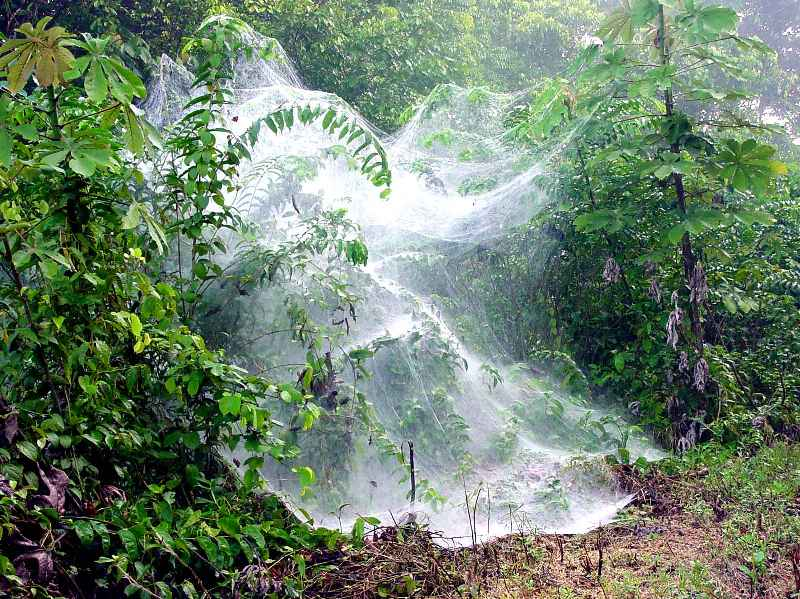
\includegraphics[width=0.7\linewidth]{../img/vibrations/toileSociale}
	\caption{Toile d'une société d'Anolesimius Eximius, espèce
		d'araignée sociale (photographie de B. \textsc{Krafft}}
	\label{fig:toileSociale}
\end{figure}


Les araignées utilisent aussi les vibrations dans la toile d'une manière
qui rappelle l'écholocation chez les chauves-souris ou les dauphins :
lorsqu'une proie se tient immobile sur la toile, l'araignée peut envoyer
une secousse dans la toile qui provoquera le balancement de la proie, et
permettra sa localisation.

Mais certaines araignées utilisent aussi à leur profit la capacité
d'autres insectes à communiquer. Par exemple, les sauterelles
communiquent normalement par sons qui se propagent dans l'air, mais
elles peuvent aussi communiquer par vibrations dans les plantes pour
éviter d'attirer les chauves-souris, ces vibrations sont utilisées par
les araignées pour localiser les sauterelles, et les chasser. De même,
l'araignée sauteuse commune, \emph{Portia fimbriata}, est capable
d'imiter les signaux vibratoires de mâles d'autres espèces d'araignée
afin d'attirer les femelles, qu'elle chasse.

\section{Production des signaux vibratoires}

Les araignées ont recours à différentes méthodes pour produire des
vibrations dans un substrat : les percussions, les vibrations du corps,
les stridulations et en tirant directement sur la toile.

\subsection{La percussion}

En frappant le sol de son abdomen ou de son pédipalpe (voir Figure 2),
l'araignée peut créer des vibrations qui se propagent dans le sol. La
force du signal vibratoire est directement lié à la masse de l'animal à
l'origine de la vibration, plus l'animal est massif et plus le rayon de
propagation est large.


\begin{figure}[htb!]
	\centering
	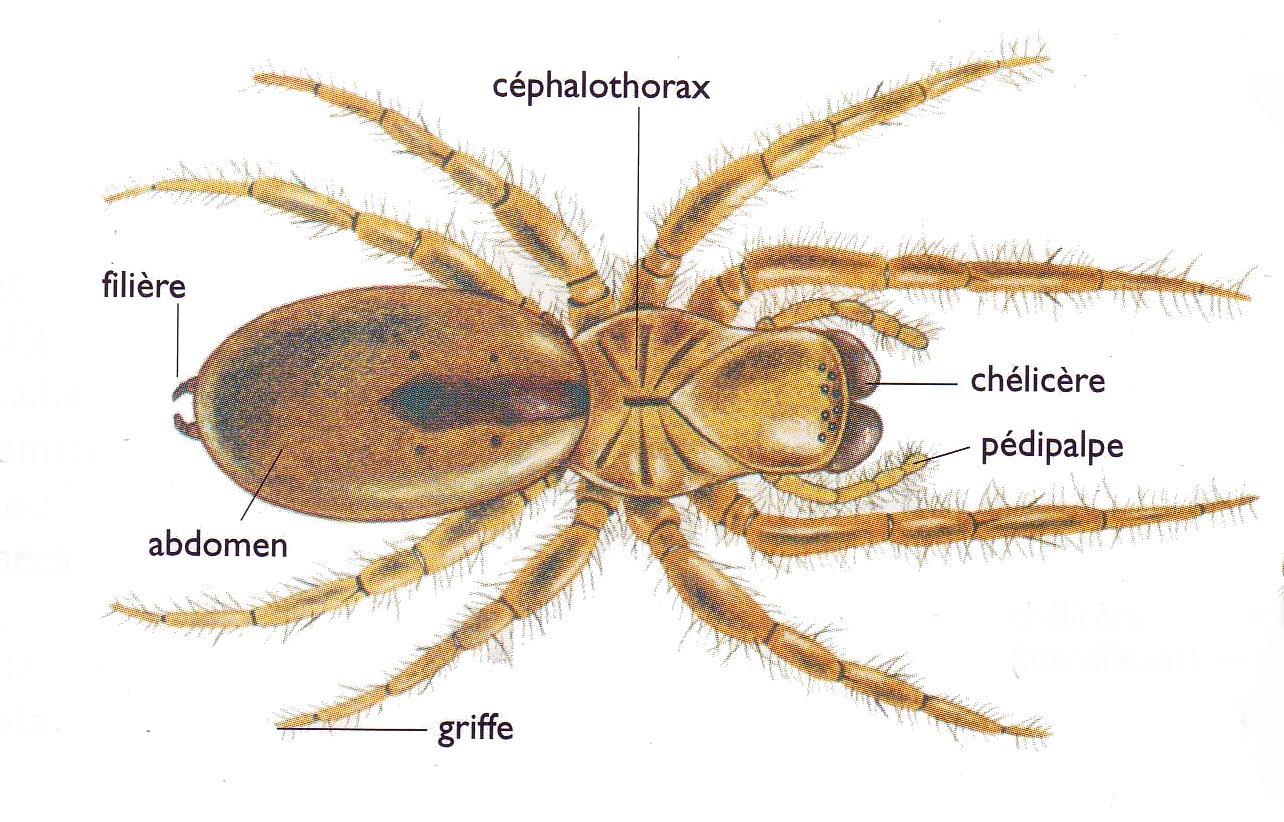
\includegraphics[width=0.7\linewidth]{../img/vibrations/anatomie_araignee}
	\caption{Anatomie d'une araignée}
	\label{fig:anatomie_araignee}
\end{figure}


Ce type d'émission est utilisé surtout par les espèces qui ne font pas
de toile, comme les araignées sauteuses (\emph{Salticidae}) ou les
araignées-loups (\emph{Lycosidae}). Ainsi, le mâle \emph{Lycosa gulosa}
produit des sons qui pourront être perçus par la femelle en frappant le
sol de ses pédipalpes.

\subsection{La trémulation}

Les araignées peuvent faire vibrer leur corps afin d'émettre des
vibrations qui passeront à travers leurs pattes puis dans le sol, c'est
ce qu'on appelle la trémulation. La trémulation ne nécessite pas une
morphologie particulière, mais la fréquence des vibrations produites est
souvent très faible, car elle est limitée par la vitesse à laquelle
l'animal peut faire vibrer son corps, dès lors, elle est donc
difficilement analysable.

\subsection{La stridulation}

Les araignées, comme certains insectes, peuvent striduler, c'est-à-dire
produire des vibrations en frottant deux parties de leur corps. Ces
vibrations sont ensuite transmises au sol par les pattes, et dans l'air
sous la forme de sons audibles. Une araignée peut striduler en frottant
son abdomen et son céphalothorax, ou en frottant différents appendices,
comme patte contre patte, patte contre pédipalpe ou chélicère contre
chélicère (voir Figure 2).

\subsection{Le tiraillement}\label{le-tiraillement}

Les araignées peuvent aussi tirer sur les fils de la toile à l'aide de
leur pattes pour y transmettre des vibrations, par exemple en exerçant
une forte traction sur la toile puis en relâchant rapidement cette
tension, envoyant un signal de grande amplitude.

\begin{figure}[htb!]
	\centering
	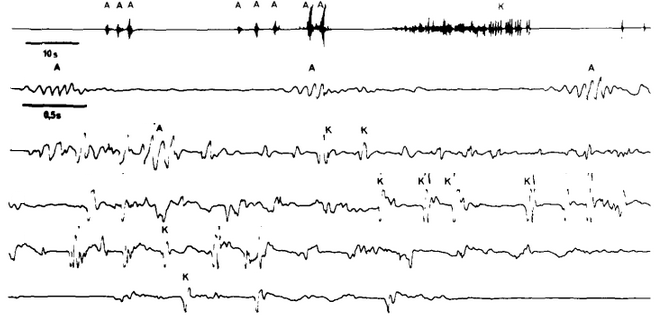
\includegraphics[width=0.7\linewidth]{../img/vibrations/SignalSpiders}
	\caption{Vibrations émises par un mâle Tegenaria parietina
		dans la toile. A : trémulations abdominales ; K : percussions avec
		l'abdomen (d'après \textsc{Leborgne} et \textsc{Krafft}, 1979)}
	\label{fig:SignalSpiders}
\end{figure}

Afin que les signaux soient reconnaissables, les araignées produisent
des vibrations caractéristiques en faisant varier la fréquence et
l'amplitude des vibrations, ainsi que la répartition de ces vibrations
au cours du temps. Nous pouvons voir cette variation du motif des
vibrations en Figure 3, on peut remarquer la répétition des trois
trémulations abdominales.

\section{Transmission du signal vibratoire}

Une fois produit par l'araignée, la vibration se propage dans le
substrat, la plupart du temps de la soie d'araignée. C'est pourquoi nous
avons effectué différentes expériences pour étudier les propriétés de la
soie d'araignée.

\subsection{Analyse microscopique}

Nous avons procédé à une analyse microscopique de fil de soie
d'araignée. Afin d'avoir les fils, nous avons capturé une araignée qui a
ensuite fait sa toile dans une boite. Grâce à un appareil photo
numérique pour microscope, nous avons pu obtenir des clichés du fil
d'araignée.

	\begin{figure}[htb!]
		\centering
		\begin{subfigure}{.5\textwidth}
			\centering
			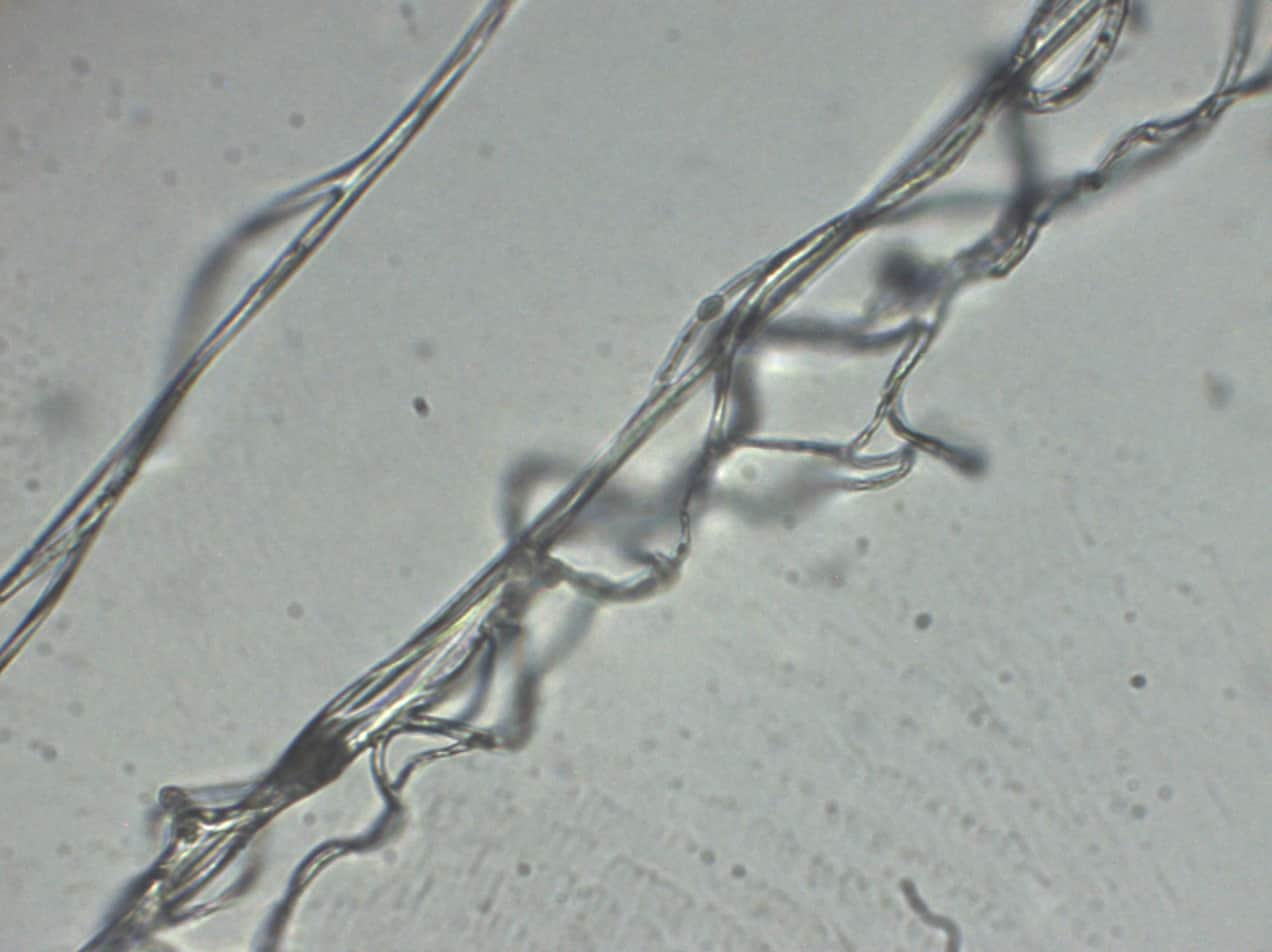
\includegraphics[width=0.8\linewidth]{../img/vibrations/FilMicroscopeA}
			\caption{}
			\label{fig:FilMicroscopeA}
		\end{subfigure}%
		\begin{subfigure}{.5\textwidth}
			\centering
			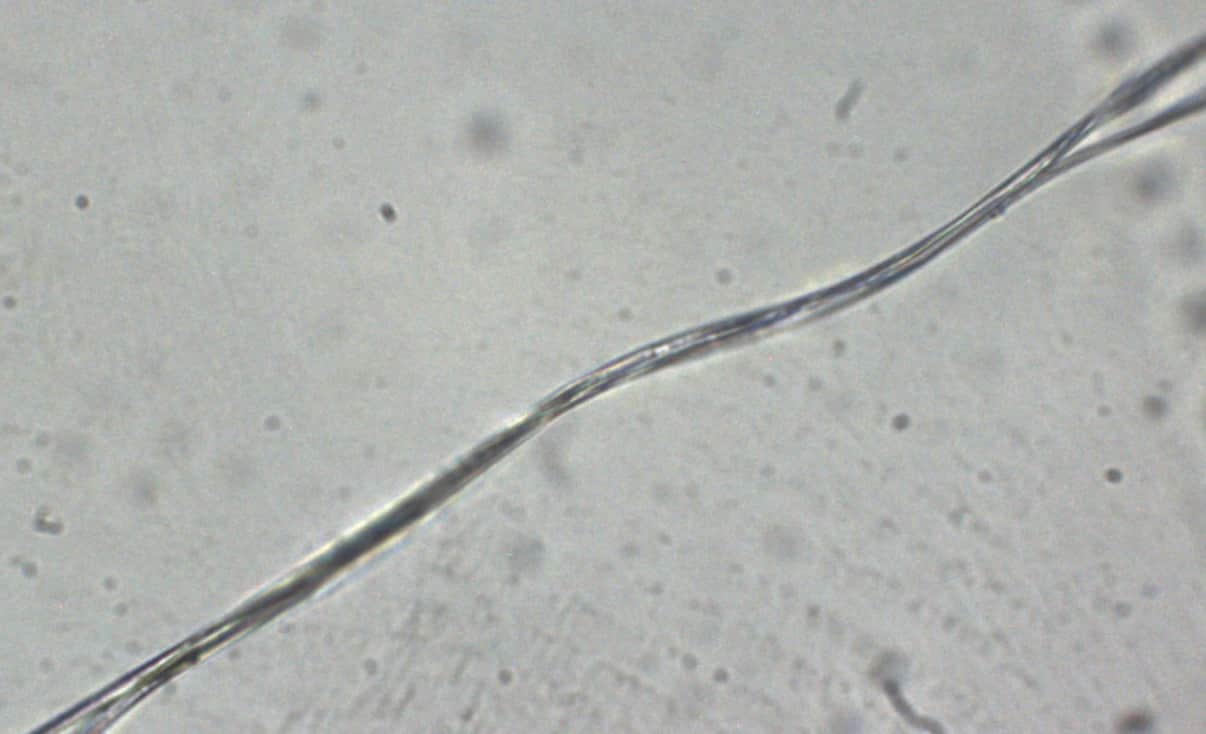
\includegraphics[width=0.8\linewidth]{../img/vibrations/FilMicroscopeB}
			\caption{}
			\label{fig:FilMicroscopeB}
		\end{subfigure}
		\caption{Photographies de fils d'araignée vus au microscope optique (×600)}
		\label{fig:test}
	\end{figure}

Le premier fil n'a pas été coloré, et le second a été coloré au bleu de
méthylène. Nous pouvons voir sur ces photographies que les fils
d'araignée sont en fait constitués de plusieurs fils tressés les uns
autour des autres, toutefois la coloration au bleu de méthylène ne
permet pas de différencier différente partie dans chacun des fils.

\subsection{Mesure de la taille d'un fil de soie d'araignée}

Afin d'étudier plus précisément le fil d'araignée, nous avons souhaité
mesurer son diamètre. Ceci est possible en analysant le phénomène de
diffraction ayant lieu lorsqu'un laser rencontre ce fil d'araignée,
c'est-à-dire la manière dont la lumière est diffusée après avoir
rencontré le fil.

Lorsqu'on projette la lumière après le fil sur un écran, on obtient des
tâches, et la taille de la tâche centrale (mesurée à partir des milieux
entre la tâche centrale et les tâches autour de la tâche centrale) est
inversement proportionnelle au diamètre du fil.

C'est pourquoi à l'aide d'un montage composé d'une diode laser, d'un
écran et d'un fil dans une diapositive positionnée entre la diode et
l'écran, à un mètre de l'écran, on peut former les tâches sur l'écran et
mesurer la taille de la tâche centrale, comme vu en Figure 5.

\begin{figure}[htb!]
	\centering
	\def\svgwidth{\columnwidth}
	\input{../img/vibrations/schemaDiffraction.pdf_tex}
	\caption{Montage pour mesurer la taille du fil de soie}
\end{figure}

Afin de pouvoir calculer le coefficient de proportionnalité entre le
diamètre du fil et l'inverse de la largeur de la tâche centrale, on
mesure la taille de la tâche centrale pour des fils de diamètre connu.
Par ailleurs on mesure la taille de la tâche centrale d'une lumière de
laser diffracté par un fil d'araignée \emph{A}, puis d'un fil \emph{B},
prélevé sur la toile de l'araignée capturée. Avec ces mesures, on
obtient le tableau suivant.

\begin{tabu}[c]{@{}rrr@{}}
	\toprule
	Diamètre fil (mm) & Largeur L de la tâche centrale (mm) & 1 /
	L\tabularnewline
	\midrule
	
	D(filA) & 1,08×102 & 9,26×10-3\tabularnewline
	D(filB) & 8,0×101 & 1,25×10-2\tabularnewline
	4,0×10-2 & 3,3×101 & 3,0×10-2\tabularnewline
	6,0×10-2 & 2,2×101 & 4,6×10-2\tabularnewline
	1,0×10-1 & 1,3×101 & 7,7×10-2\tabularnewline
	1,2×10-1 & 1,1×101 & 9,1×10-2\tabularnewline
	\bottomrule
\end{tabu}

Ces mesures permettent de tracer un graphique. La proportionnalité entre
le diamètre du fil et la taille de la tâche centrale est modélisée par
une droite de coefficient directeur 0,76 et passant par l'origine du
repère.

\begin{figure}[htb!]
	\centering
	\def\svgwidth{\columnwidth}
	\input{../img/vibrations/graphiqueDiffraction.pdf_tex}
	\caption{\(1 / L\) en fonction du diamètre du fil}
\end{figure}

Dès lors on peut calculer :

\( D(fil) = \frac{\frac{1}{L}}{0.76}\)

Donc: 
\(D(filA) = \frac{9,26\times10^{-3}}{0.76}\)


\(D(filA) = 1,2\times10^{-2} \text{mm} = 1,2\times10^{-5} \text{m} = 12 \mu\text{m}\)

Et,

\(D(filB) = \frac{1,25\times10^{-2}}{0.76}\)


\(D(filB) = 1,6\times10^{-2} \text{mm} = 1,6\times10^{-5} \text{m} = 16 \mu\text{m}\)

Ainsi, selon nos mesures un fil de soie d'araignée a une taille moyenne
de \( \bar{x} = \frac{D(filA) + D(filB)}{2} = \frac{12 + 16}{2} = 14 \mu\text{m}\), soit environ un dixième de la taille d'un cheveu.

Ainsi, même si le fil de soie d'araignée est extrêmement fin, les
araignées sont capables de construire des toiles résistantes au poids de
l'araignée elle-même, à celui d'éventuels intrus et à la transmission
d'ondes, notamment dans le cadre de la communication.

\subsection{Vitesse d'une onde dans la toile}

Les vibrations émises par l'araignée prennent la forme d'ondes
mécaniques progressives dans la toile, c'est-à-dire la propagation d'une
perturbation dans un milieu matériel sans transport de matière. Cette
onde est dite à une dimension puisqu'elle ne se propage que dans une
seule direction.

Afin d'étudier la vitesse d'une onde dans la toile, nous avons décidé de
nous intéresser à la vitesse d'une onde dans une corde. Pour cela nous
avons mesuré le temps que prenait une onde pour parcourir un mètre sur
deux cordes, corde A et corde B à l'aide de deux capteurs laser, en
tendant plus ou moins la corde, comme vu en Figure 7.

\begin{figure}[htb!]
	\centering
	\def\svgwidth{\columnwidth}
	\input{../img/vibrations/schemaVOnde.pdf_tex}
	\caption{Montage pour mesurer la vitesse de propagation d'une onde dans une corde}
\end{figure}

Corde A :

Masse de la corde : \(m_A = 4,6\times10^{-2} \text{kg}\)

Longueur de la corde : \(L_A = 2,08 \text{m}\)

Masse linéique (masse par unité de longueur) :

\(\mu_A = \frac{m}{L} = \frac{4,6\times10^{-2}}{2,08} = 2,2\times10^{-2} \text{kg.m}^{-1}\)
\begin{table}
	\centering
	\begin{tabu}[c]{@{}llllll@{}}
		\toprule
		Tension & A & B & C & D \tabularnewline
		\midrule
		& 24 & 19 & 10 & 5 \tabularnewline
		
		& 22 & 18 & 13 & 4 & \  \tabularnewline
		& 26 & 15 & 6 & 7 & \  \tabularnewline
		& 26 & 15 & 9 & 4 & \  \tabularnewline
		& 20 & 15 & 11 & 9 & \  \tabularnewline
		& 28 & 22 & 7 & 6 & \  \tabularnewline
		& 23 & 15 & 9 & 6 & \  \tabularnewline
		& 17 & 14 & 10 & \  & \  \tabularnewline
		& 8 & \  & \  & \  & \  \tabularnewline
		& 5 & \  & \  & \  & \  \tabularnewline
		\midrule
		Moyenne & 24 & 17 & 9.2 & 6 \tabularnewline
		\bottomrule
		
		
	\end{tabu}
	\caption {Durée Δt (s) que prend la vibration à parcourir un mètre sur la corde A en fonction de la tension (avec A<B<C<D)}
\end{table}



Corde B :

Masse de la corde : \(m_B = 2,1\times10^{-1} \text{kg}\)

Longueur de la corde : \(L_B = 3,07 \text{m}\)

Masse linéique (masse par unité de longueur) :
\(\mu_B = \frac{2,1\times10^{-1}}{3,07} = 7,0\times10^{-2} \text{kg.m}^{-1} > \mu_A\)
\begin{table}
	\centering
	\begin{tabu}[c]{@{}llll@{}}
		\toprule
		Tension & A' & B' &  \tabularnewline
		\midrule
		& 30 & 28 & \  \tabularnewline
		& 35 & 31 & \  \tabularnewline
		& 39 & 35 & \  \tabularnewline
		& 30 & 23 & \  \tabularnewline
		& 35 & 17 & \  \tabularnewline
		& 41 & 35 & \  \tabularnewline
		& 36 & 27 & \  \tabularnewline
		& 45 & 33 & \  \tabularnewline
		& 37 & 37 & \  \tabularnewline
		& 37 & 37 & \  \tabularnewline
		\midrule
		Moyenne & 36.5 & 30.3 & \  \tabularnewline
		\bottomrule
	\end{tabu}
	\caption {Durée Δt (s) que prend la vibration à parcourir un mètre sur la corde B en fonction de la tension (avec A'<B')}
\end{table}




Dès lors on peut remarquer que plus la tension de la corde est élevée,
et plus la propagation se déplace rapidement dans la corde, et plus la
corde a une masse linéique élevé, et plus la propagation se déplace
lentement.

Le calcul théorique de la vitesse \(v\) d'une onde dans une corde est
\(v = \sqrt{\frac{T}{\mu}}\), où \(T\) est la tension de la corde et
\(\mu\) sa masse linéique, ce qui est en accord avec nos observations.

Selon
\href{http://web.mit.edu/course/3/3.064/www/slides/Ko_spider_silk.pdf}{une
étude menée conjointement par des universités américaines et
japonaises}, la masse linéique d'une fibre de soie d'araignée est
\(\mu_{fibre} = 1,4\times10^{-8} \text{kg.m}\)-1, même s'il est composé
de plusieurs fibres, le fil de soie d'araignée a une masse linéique
extrêment faible. Par ailleurs, la toile est sous tension. Les ondes se
déplacent donc extrêmement rapidement dans la toile, ce qui est un des
atouts majeurs de la communication vibratoire pour les araignées.

\section{Perception des signaux vibratoires}

Les araignées perçoivent très bien les signaux vibratoires, en effet,
elles sont dotées de différents organes leur permettant de recevoir des
vibrations, notamment les trichobotries et les sensilles en fente, ce
sont les organes mécanorécepteurs.

\subsection{Les trichobotries}

Les trichobotries sont des soies sensorielles fines, longues et
extrêmement mobiles insérées dans une cupule (une petite structure de la
forme d'une coupe), et reliées à un nerf par un dendrite, une courte
extension des cellules nerveuses (voir Figure 8).

\begin{figure}[htb!]
	\centering
	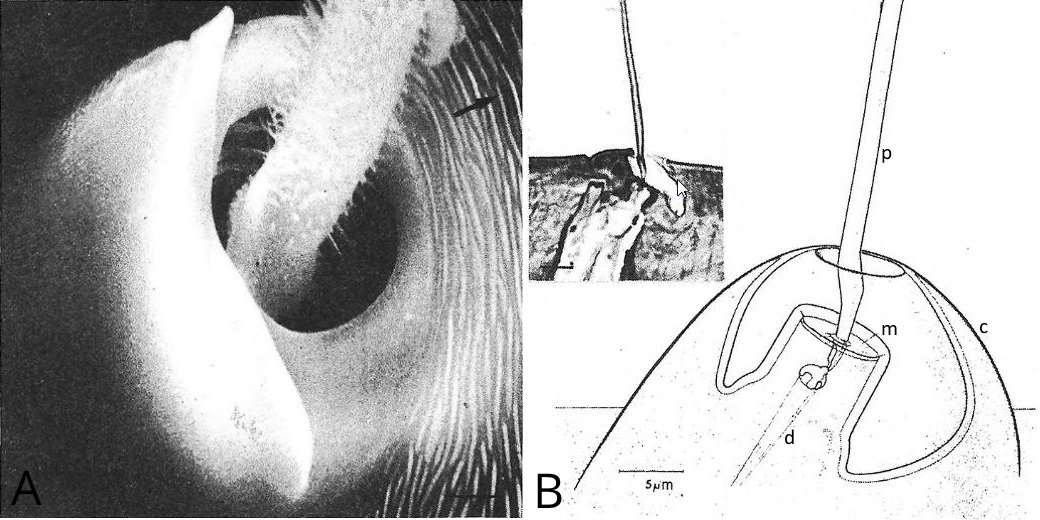
\includegraphics[width=0.7\linewidth]{../img/vibrations/trichobotrie}
	\caption{A : Base d'une trichobotrie, montrant la cupule et
		la structure plumeuse du poil ; B : Structure d'une trichobotrie (p :
		poil, c : cupule, m : membrane, d : dentrite)}
	\label{fig:trichobotrie}
\end{figure}


Les trichobotries sont disposées sur les pattes et les pédipalpes de
l'araignée. Ayant une masse très faible, étant extrêmement flexible et
étant en contact avec l'air autour de l'araignée, les trichobotries
permettent la détection de mouvement dans l'air, mais aussi dans le
substrat.

\subsection{Les sensilles en fente}

Les sensilles en fente sont des petits organes mécanorécepteurs qui
peuvent détecter la déformation ou la tension. Elles se situent sur
l'intégralité de l'exosquelette (aussi appelé cuticule) de l'araignée,
et notamment sur les pattes. Leur apparence de fente est à l'origine de
leur nom, mais elles ne pénètrent en fait pas l'exosquelette, elles
correspondent à un amincissement de la cuticule.

Elles prennent la forme de petites fentes de 1 à 2µm de large et entre 8
et 200µm de long, et peuvent être situées seules ou en groupe (voir
Figure 9). Un groupe de sensilles en fente est appelé un organe
lyriforme, car, les fentes étant parallèles entre elles, il a la forme
d'une lyre, et une sensille en fente seule est appelé sensille en fente
simple.

\begin{figure}[htb!]
	\centering
	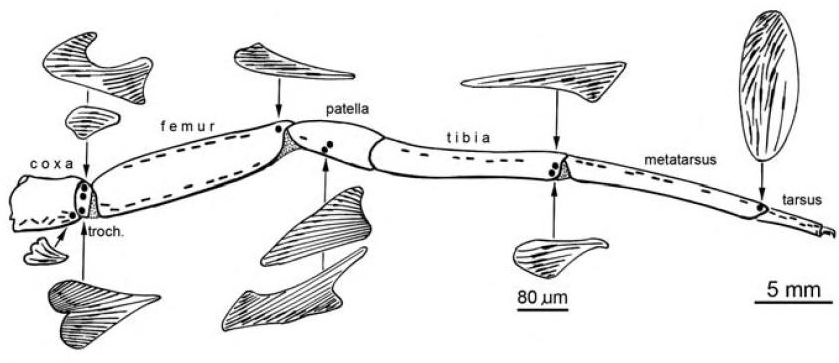
\includegraphics[width=0.7\linewidth]{../img/vibrations/Sensilles}
	\caption{Distribution des sensilles en fente sur l'arrière
		de la première patte d'une Cupiennus salei : les traits indiquent des
		sensilles en fente seule, et les points des organes lyriformes (enlargis
		pour voir les détails) (d'après \textsc{Barth} et \textsc{Libera},
		1870)}
	\label{fig:Sensilles}
\end{figure}

La fente est bordée d'une lèvre cuticulaire et est recouverte d'une
membrane cuticulaire. Sous la membrane, une sorte de gouttière s'étend
vers le bas et s'élargit en prenant la forme d'une cloche, où se
trouvent deux dendrites qui relient la sensille en fente au nerf (voir
Figure 10). Même une tension très faible au niveau de la cuticule
causera une déformation de la sensille, et la membrane se pliera,
déformant l'extrémité d'une des dendrites, provoquant un signal nerveux.

\begin{figure}[htb!]
	\centering
	\def\svgwidth{\columnwidth}
	\input{../img/vibrations/Sensilles2.pdf_tex}
	\caption{Schéma d'une sensille simple d'une Cupiennius (d'après \textsc{Barth}, 1971}
\end{figure}

C'est en analysant la différence de temps entre l'arrivée de la
vibration dans ses différentes pattes que l'araignée peut déterminer la
direction de la proie ou de l'intrus.

\section{Utilisation des connaissances en matière de communication vibratoire}

\subsection{Dans la lutte intégrée}

Les connaissances en matière de communication vibratoire peuvent être
utilisé de différentes manière. En effet, en étant capable de reproduire
ou d'imiter des signaux vibratoires, il est possible d'agir sur le
comportement des animaux ayant recours à ce type de communication. Ceci
est intéressant notamment dans le cadre de la lutte intégrée, définie en
Europe par la directive communautaire 91/414/CEE du 15 juillet 1991
ainsi :

\begin{quote}
« L'application rationnelle d'une combinaison de mesures biologiques,
biotechnologiques, chimiques, physiques, culturales ou intéressant la
sélection des végétaux dans laquelle l'emploi de produits chimiques
phytopharmaceutiques est limité au strict nécessaire pour maintenir la
présence des organismes nuisibles en dessous de seuil à partir duquel
apparaissent des dommages ou une perte économiquement inacceptables. »
\end{quote}

Ainsi, il serait possible de contrôler sans utiliser de pesticides des
populations d'insectes nuisibles ayant recours à la communication
vibratoire, comme la cicadelle de la vigne (\emph{Scaphoideus titanus}).
Les cicadelles n'utilisent pas de communication chimique à longue
portée, mais peuvent transmettre des signaux vibratoires à travers les
feuilles de vigne jusqu'à plusieurs mètres de distances. Or, la
cicadelle de la vigne est officiellement reconnue comme \emph{nuisible}
car elle est responsable de la propagation de la flavescence dorée,
maladie à l'origine de pertes importantes de récoltes de vignes, et son
contrôle est donc obligatoire.

Dans son article
\href{http://journals.plos.org/plosone/article?id=10.1371/journal.pone.0032954}{«
Exploitation of Insect Vibrational Signals Reveals a New Method of Pest
Management »}, Anna \textsc{Eriksson} (et al.) étudie l'utilisation de
vibrations pour perturber la communication entre mâles et femelles
\emph{Scaphoideus titanus} en envoyant des signaux pré-enregistrés que
les mâles \emph{Scaphoideus titanus} utilisent pour empêcher les autres
mêles de s'accoupler.

\begin{figure}[htb!]
	\centering
	\def\svgwidth{\columnwidth}
	\input{../img/vibrations/graphiqueLutteIntegree.pdf_tex}
	\caption{Nombre de femelles non fécondées trouvées sur les feuilles de vigne (A) sur des plantes en pot, (B) dans un champ de vigne, selon la distance de la source de vibrations.},
\end{figure}

Après avoir effectué et analysé des essais, elle a obtenu des résultats
concluants que cette méthode de contrôle est très efficace (voir Figure
11) : même lorsque la source de vibration se trouve à 940cm, plus de 80
\% des femelles restent non fécondées, alors que dans le cas du groupe
contrôle (non montré sur le graphique) seuls 20 \% des femelles
restaient non fécondées.

Cette méthode agit donc fortement sur la population, car non seulement
elle empêche la fécondation d'une grande partie des femelles, mais elle
retarde de plus les fécondations ayant lieu, la femelle est donc moins
féconde qu'elle ne l'aurait été. Ainsi, l'utilisation de signaux
vibratoires pour perturber la reproduction s'accorde bien à la
définition de la lutte intégrée, car en empêchant, ou du moins en
retardant la fécondation, elle permet de diminuer la population de
nuisible sans l'exterminer, tout en limitant l'utilisation de produits
chimiques.

Toutefois, dans
\href{http://onlinelibrary.wiley.com/enhanced/doi/10.1002/ps.3848}{une
étude plus récente} Jernej \textsc{Polajnar}, Anna \textsc{Eriksson} et
al. ont mis en évidences l'existence d'effets secondaires causés par la
production de signaux vibratoires, notamment la perturbation d'insectes
non nuisibles comme les abeilles ou les araignées.

De plus, ils soulignent les limitations techniques de cette méthode :
l'atténuation des vibrations est extrêmement rapide dans la plupart des
milieux solides. Toutefois certains insectes ont surmonté cette
difficulté en produisant des vibrations proches de fréquences
résonnantes du substrat, c'est-à-dire les fréquences auxquelles le
substrat est sensible, et qui, répétés sous forme périodique, provoquera
l'accumulation d'énergie dans le substrat jusqu'à atteindre un régime
d'équilibre. Il est donc possible d'imiter les fréquences utilisées par
les insectes pour diminuer l'importance du problème d'atténuation.

Par ailleurs, la situation du champ de vignes étudiés par Anna
\textsc{Eriksson} était une situation idéale, car les vignes forment une
ligne et chaque pied de vigne est relié au suivant, facilitant la
transmission de vibrations d'un pied de vigne au suivant. Dès lors, on
peut se demander si cette méthode est vraiment applicable


\subsection{Bibliographie}

	
	\section*{Conclusion}
\addcontentsline{toc}{section}{\protect\numberline{}Conclusion}%
	
	
	%\nocite{*}
	%\printbibliography
\end{document}